\documentclass[10pt]{article}
\usepackage{amsthm}
\usepackage{graphicx}
\usepackage{subfig}
\usepackage{physics}

\graphicspath{ {figures/} }
\begin{document}

The Monte Carlo simulation models a layered AFM insulator with four antiferromagnetically coupled layers, each composed of $40 \times 40$ spins. A single-spin Metropolis algorithm is used and energy
fluctuations are determined by the system Hamiltonian,
$$H = -J_{FM}\sum_{l}\sum_{<i,j>}\vec{S}_{l,i}\cdot \vec{S}_{l,j} + \sum_{l < N}J_{AFM,l}\sum_{i}\vec{S}_{l,i} \cdot \vec{S}_{l+1,i} + \sum_{l,i}K_{l}\left (S_{l,i,z}\right )^{2} - B \sum_{l,i}S_{l,i,z}$$
where $\vec{S}_{l,i}$ is the spin unit vector residing on site $i$ of layer $l$. The $J_{FM}$ term characterizes intra-layer
ferromagnetic interactions and the $J_{AFM,l}$ term characterizes antiferromagnetic coupling between layers $l$ and $l+1$. The $K_{l}$ term describes
easy-axis anisotropy (for $K_{l} < 0$) and the $B$ term describes Zeeman coupling.
In our simulations, $J_{FM} = 1$ and magnetization per spin is calculated by averaging the $S_{i,z}$ components of all spins.
When sweeping the magnetic field strength, magnetization per spin is measured over the entire system as well as on each individual layer. Mean magnetization per spin measurements
are calculated by averaging the mean $S_{i,z}$ value over 1000 ensembles at the indicated external field strength.

As mentioned in the main text, applying a gate voltage to the top or bottom of the system breaks inversion symmetry. This effect is modeled in our simulation
by adjusting the anisotropy $K$ or interlayer coupling strength $J_{AFM}$ on the top and bottom layers. When sweeping the magnetic field strength in a system that exhibits
inversion symmetry (i.e. uniform parameters throughout every layer), we observe all of the patterns of Figure 1 with equal probability.

\begin{figure}[!htb]
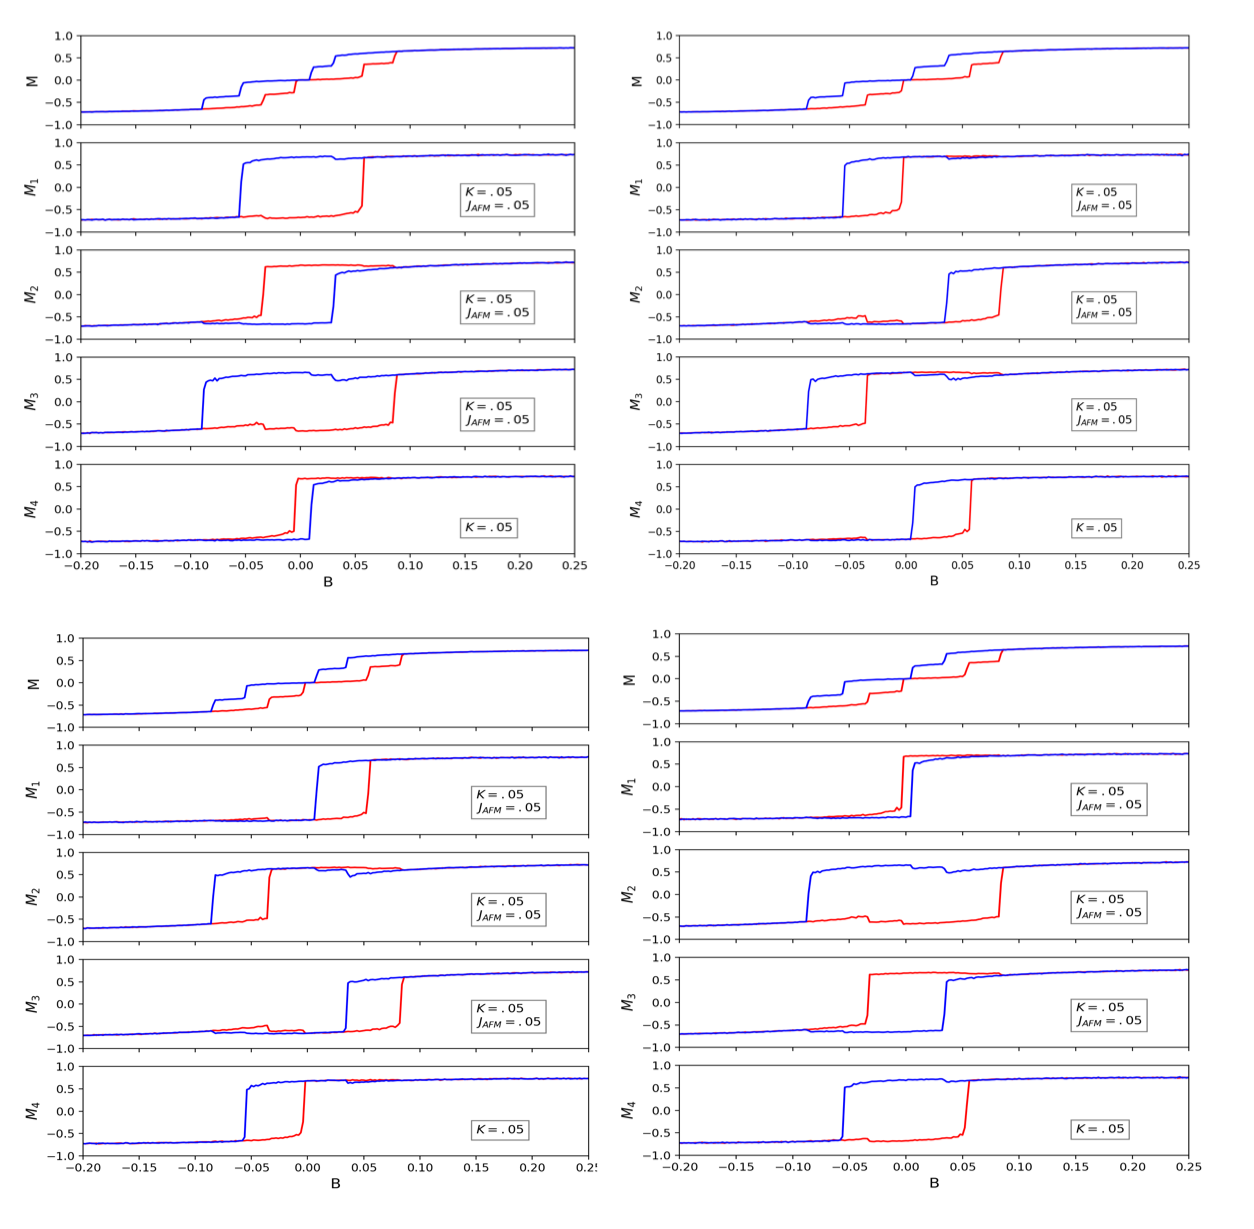
\includegraphics[width=\textwidth]{4_patterns_new.png}
\caption{Magnetization versus magnetic field strength $B$ for the total system, $M$, and each of the individual layers, $M_{i}$. Shown are the four possible switching patterns obtained for a symmetric
system when sweeping the magnetic field. The red line indicates sweeping of the magnetic field strength in the positive direction, and the blue line indicates
sweeping in the negative direction. All results presented are for four square lattice layers of $40 \times 40$ spins each at $T = .15$. The anisotropy strength $K$ and the antiferromagnetic coupling $J_{AFM}$
are shown in the inset of the individual layer plots, where $J_{AFM}$ displayed on the plot for layer $i$ refers to the coupling between layers $i$ and $i+1$.  }
\end{figure}

\pagebreak
One possible approach for breaking inversion symmetry is to modify the anisotropy $K$ on a single layer. An example of this approach, where $K_{1}$ is increased from $.05$ to $.08$, is shown in Figure 2. In increasing the anisotropy on the top layer, we observe behavior similar to that shown in Figure 2(b) in the main text. That is,
when reversing the sweeping direction, the preferred bistable state in the intermediate magnetic field region is switched. The observed states for this case are enumerated in Figure 3. We can obtain similar behavior by increasing $J_{AFM}$ between the top two layers. An example of this scenario is shown in Figure 4, where $J_{AFM}$ is increased from $.05$ to $.08$ between the top two layers only.

\begin{figure}[!htb]
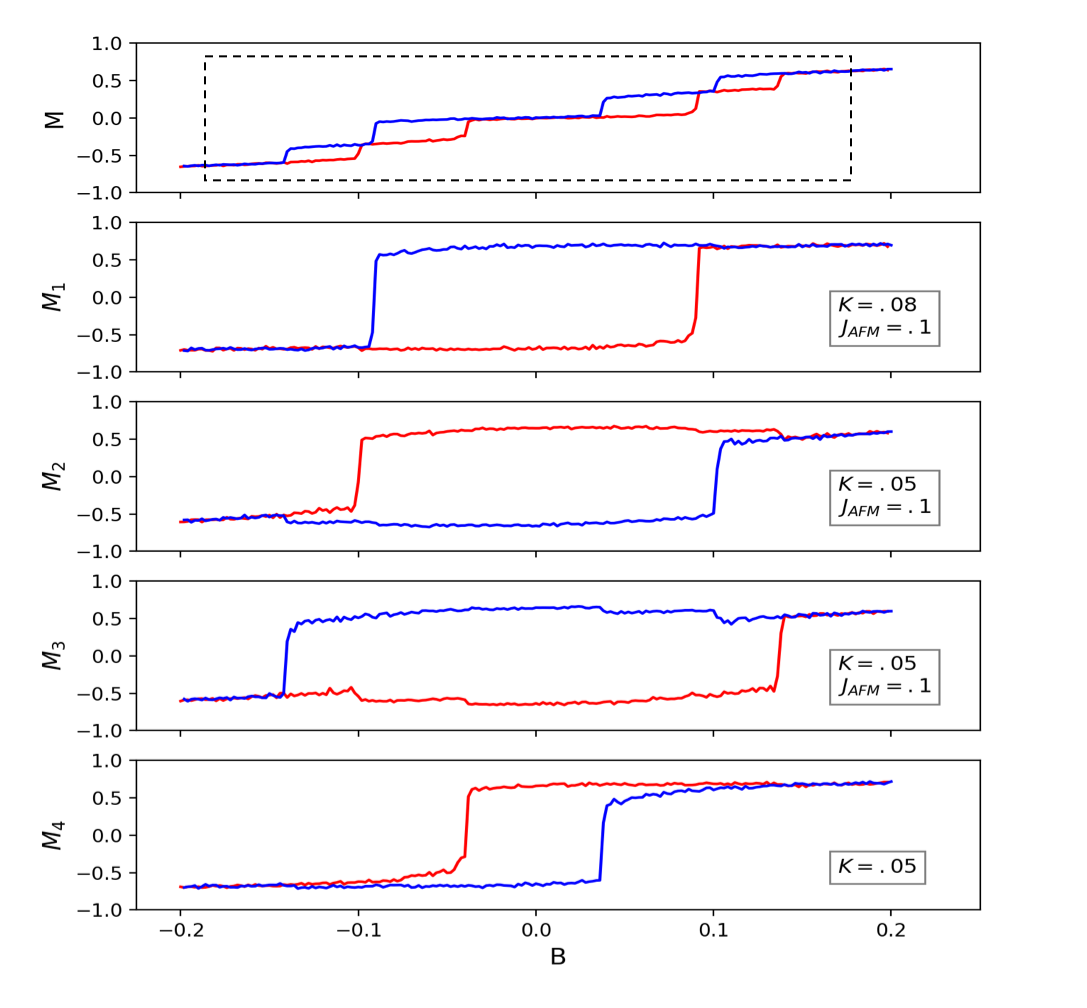
\includegraphics[width=\textwidth]{bistable_new_2.png}
\caption{The anisotropy of the top layer is increased slightly to $K_{1} = .08$ while the other layers have an anisotropy of $K = .05$. The values of
$J_{FM}$ and $J_{AFM}$ are uniform throughout the system. The states observed in each intermediate field region within the dashed lines are shown in Figure 3. }
\end{figure}
\begin{figure}[!htb]
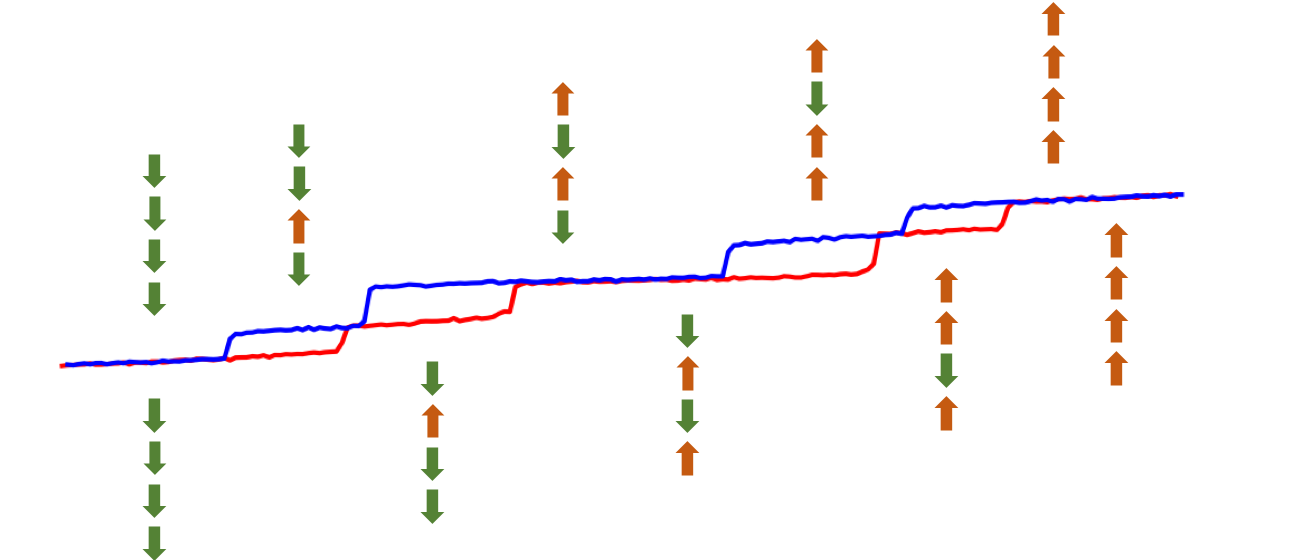
\includegraphics[width=\textwidth]{bistable_new_inset.png}
\caption{The preferred states observed in the dashed line region of Figure 2. States observed during the positive sweep are shown below the plot, and states observed during the negative sweep are shown above.
In the positive intermediate field region, for example, we see that $\uparrow \downarrow \uparrow  \uparrow$ is preferred during a negative sweep while
$\uparrow \uparrow \downarrow  \uparrow$  is preferred during a positive sweep. }
\end{figure}

\begin{figure}[!htb]
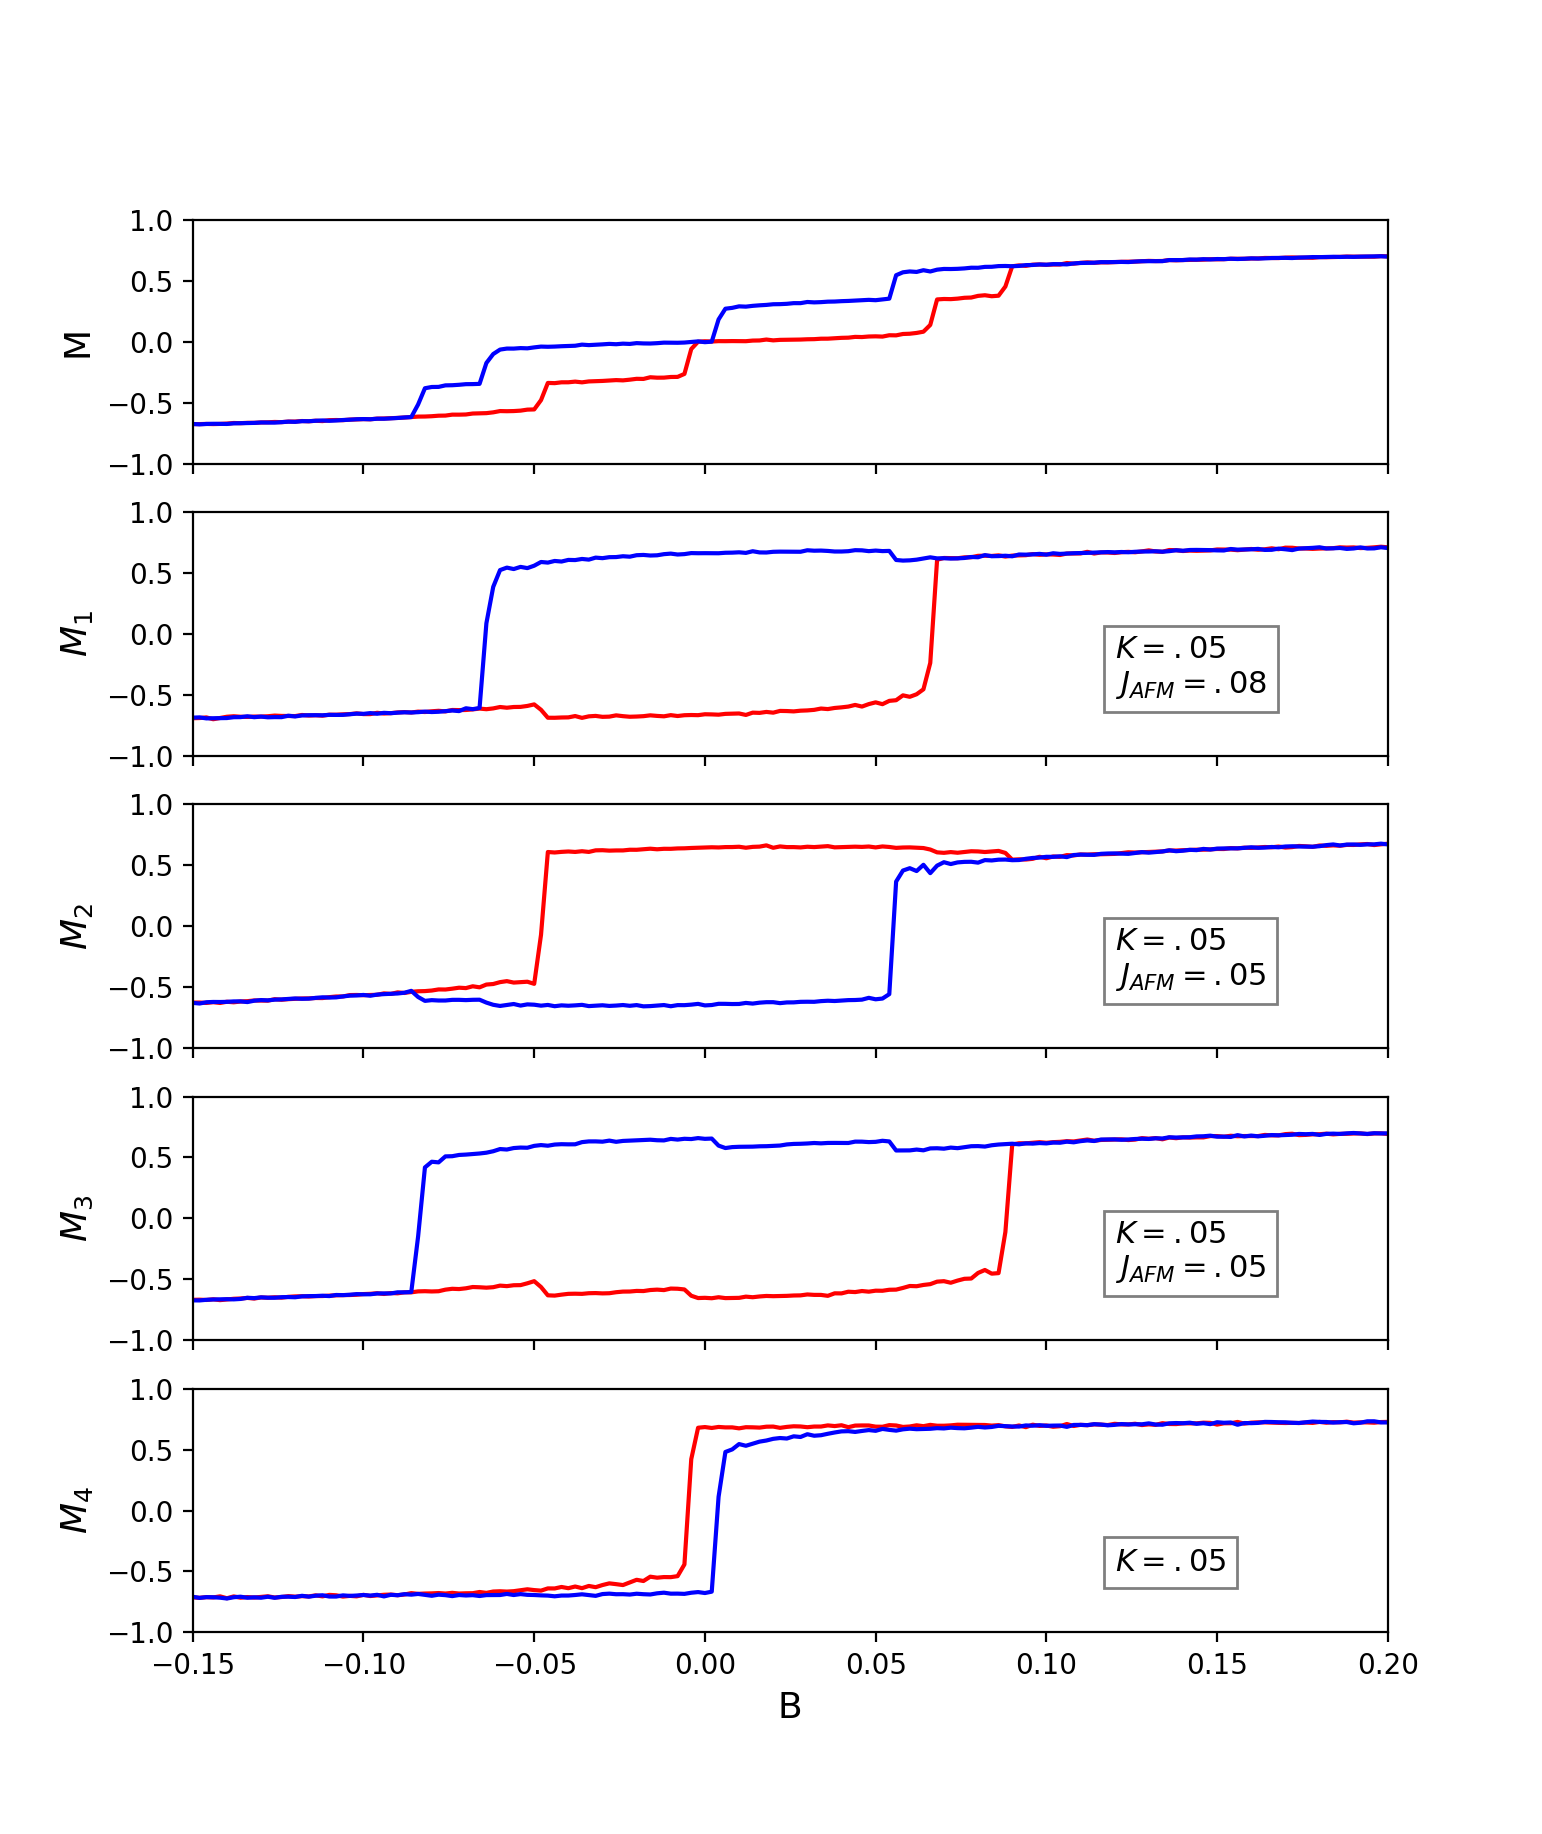
\includegraphics[width=\textwidth]{j_increase.png}
\caption{The interlayer coupling of the top two layers is increased to $J_{AFM} = .08$ while the other two interlayer couplings are kept at $J_{AFM} = .05$. The values of
$K$ and $J_{AFM}$ are uniform throughout the system. }
\end{figure}

\pagebreak

\pagebreak
If we increase the interlayer coupling strength in addition to breaking the symmetry of the system, we begin to see a shift from the behavior described in Figure 2(b) of the main text to that of Figure 2(a) or 2(c). That is,
the preferred bistable state in a subset of the intermediate magnetic field region will no longer depend on the sweeping direction. As an example, if we increase $J_{AFM}$ to $.3$ between the
top two layers (Figure 5), the results of sweeping the magnetic field become similar to those obtained in Figure 2(c) of the main text.
In particular, we observe that $\uparrow \downarrow \uparrow \uparrow$ is preferred in a small positive intermediate field region during both the positive
and negative sweep of the magnetic field. Another example of this behavior is also shown in Figure 5 for an increased anisotropy on the top layer.

\begin{figure}[!htb]
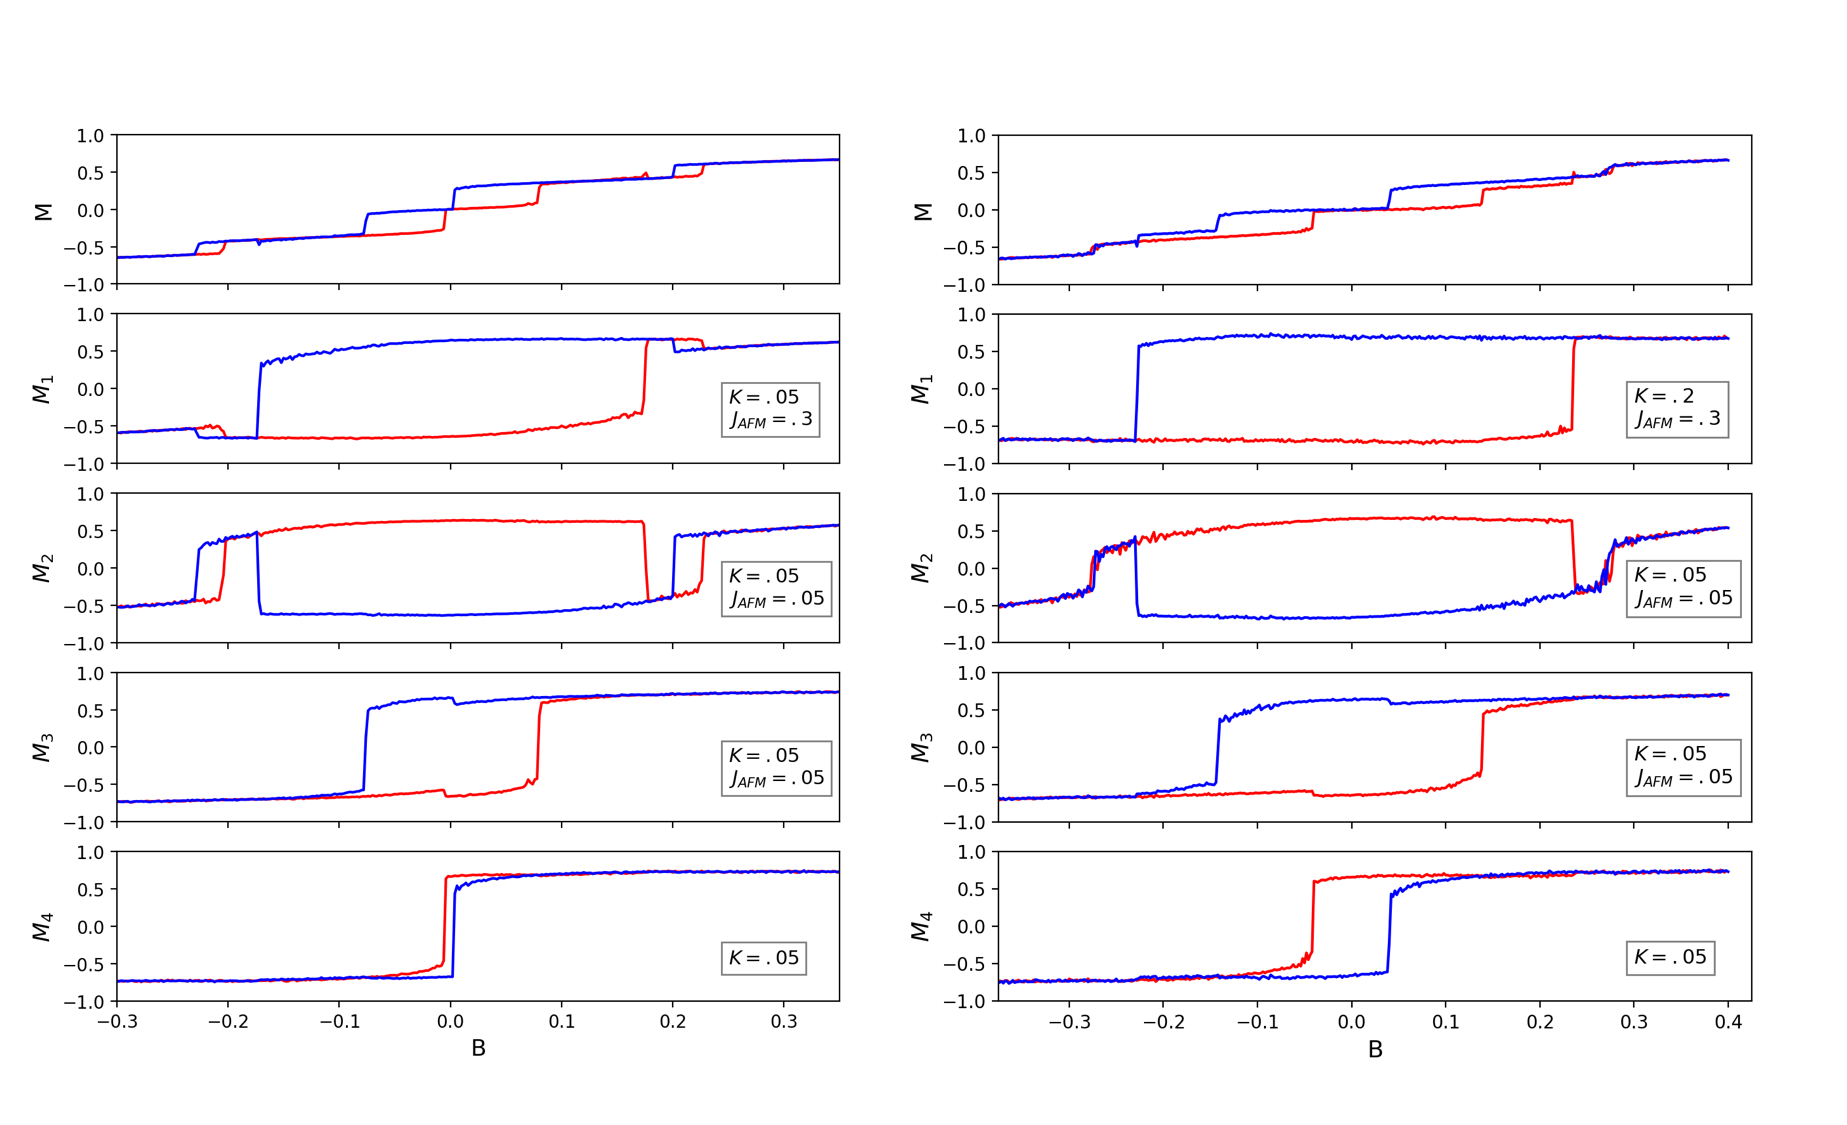
\includegraphics[width=\textwidth]{strong.png}
\caption{In this simulation, the interlayer coupling strength of the top two layers is increased significantly to $J_{AFM,12} = .3$ while the other layers have a coupling strength of $J_{AFM} = .05$. The values of
On the left, $J_{FM}$ and $K$ are uniform throughout the system. On the right, the anisotropy $K$ is also increased on the top layer. }
\end{figure}


\pagebreak
We now turn to a simulated demonstration of controlled switching between bistable states. Consider the results presented in Figure 2. The bistable states present in the positive intermediate field region are highlighted in Figure 6.
We see that the $\uparrow \uparrow \downarrow \uparrow$ state is preferred during the positive sweep of the magnetic field, while  $\uparrow \downarrow \uparrow  \uparrow$ is preferred during the negative sweep. We also note that the
intermediate field region where the bistable states are encountered is bounded by two critical field values $B_{0}$ and $B_{0}'$. By initially sweeping the magnetic field from some large positive value (where
$\uparrow \uparrow \uparrow  \uparrow$ is guaranteed) to $B_{0} + \Delta$, we can obtain the initial bistable state $\uparrow \downarrow \uparrow \uparrow$. If $\Delta$ is small, we can then fix the
magnetic field strength at $B_{0} + \Delta$, which is very near the critical field value $B_{0}$. By then sweeping the overall anisotropy strength, we can shift the critical switching field, moving the
system temporarily out of the intermediate field region. As we approach the critical field from the positive sweeping direction, the preferred bistable state switches to
$\uparrow \uparrow \downarrow  \uparrow$. This process is demonstrated in Figure 7.

\begin{figure}[!htb]

  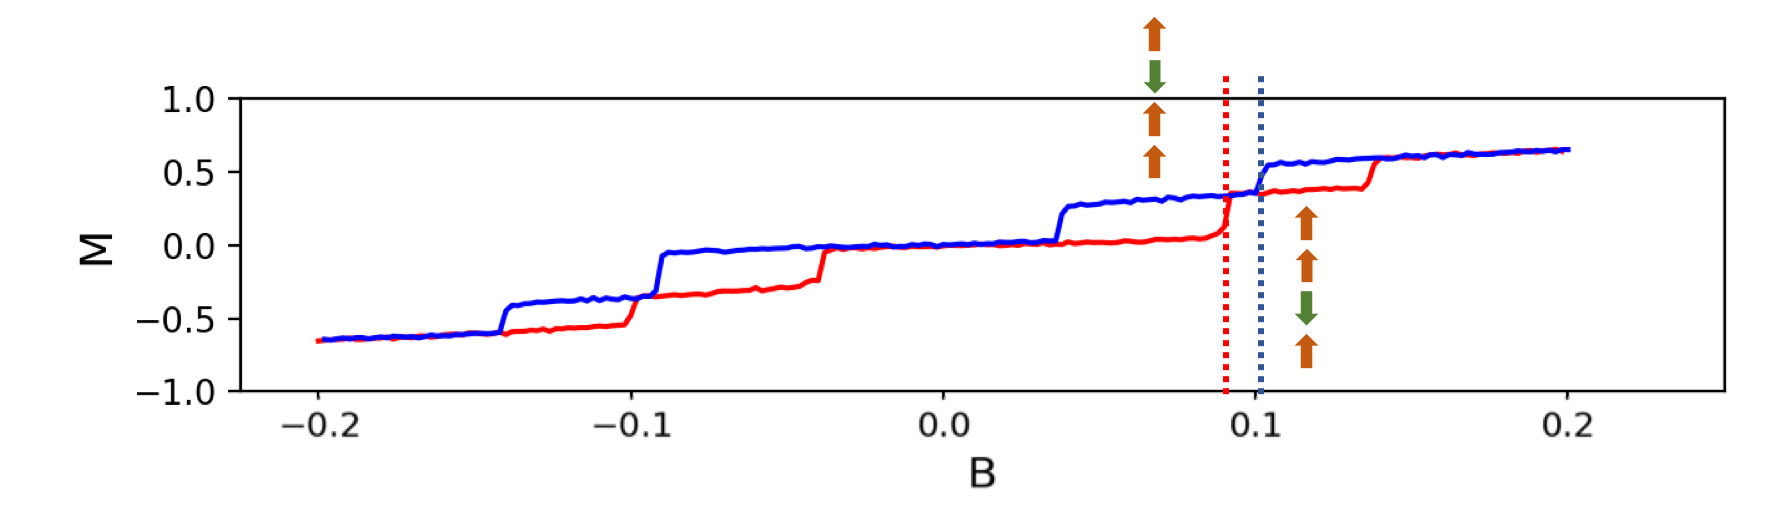
\includegraphics[width=\textwidth]{bistable_switch.png}

\caption{We see that the $\uparrow \uparrow \downarrow \uparrow$ state is preferred during the positive sweep of the magnetic field, while  $\uparrow \downarrow \uparrow  \uparrow$ is preferred during the negative sweep. The critical field values $B_{0}$ and $B_{0}'$ that
bound the positive intermediate field region where these states are present are indicated by red and blue dashed lines, respectively. }
\end{figure}

\begin{figure}[!htb]

  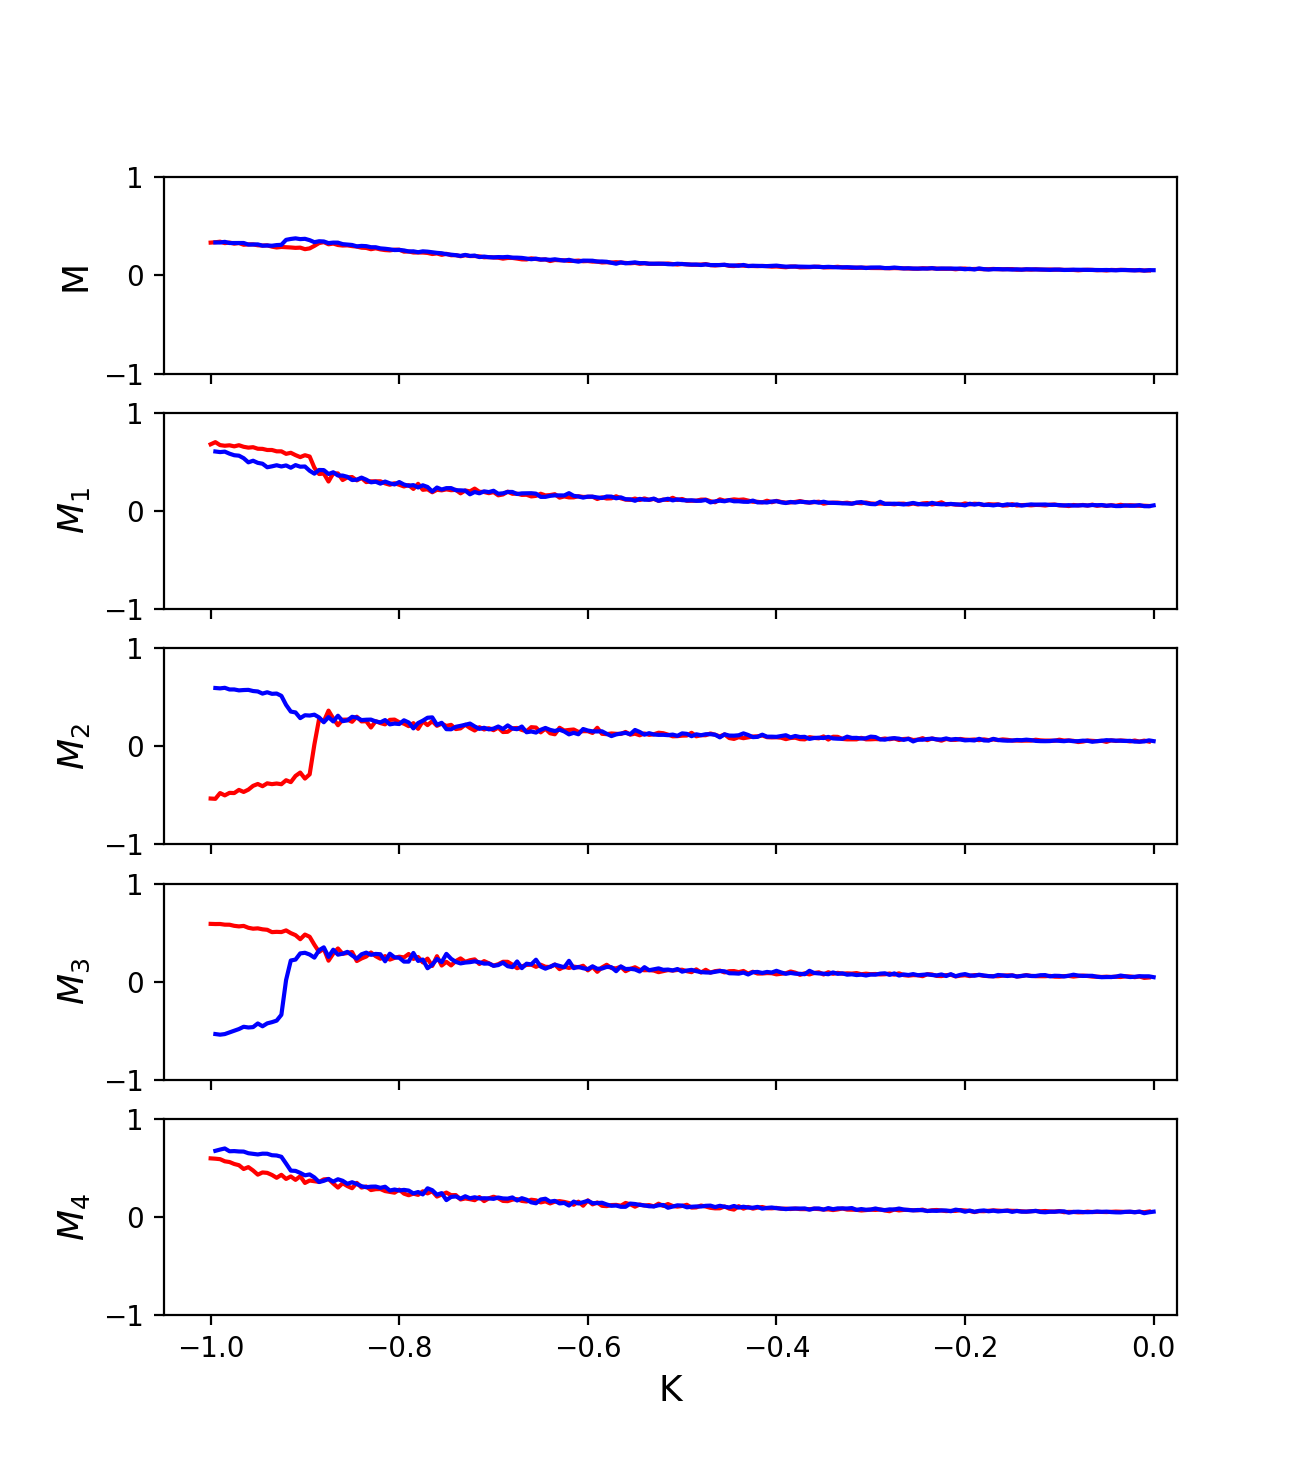
\includegraphics[width=\textwidth]{switch_states.png}

\caption{By sweeping the overall anisotropy, we are able to perform a controlled switch between bistable states as the magnetic field is fixed at $B = .09$. The system is initially in the state
$\uparrow \downarrow \uparrow \uparrow$, but after sweeping the anisotropy, we obtain the state $\uparrow \uparrow  \downarrow \uparrow$. }
\end{figure}

\end{document}



%%As mentione din the main text, top and bottom gate break inversion symmetry, which in our simulation can be simulated by adjusting the anisotropy and interlayer coupling strength. Breaking intralayer symmetry
%%By changing either inter or anisotropy we can reproduce the pattern seen in B. To realize 2a or c, we can to combine the symmetry breaking effects. Finally we tried changing intra layer to see.
